\addtocontents{toc}{\protect\setcounter{tocdepth}{-1}}
\chapter{Documentación de control}
\section{\textit{Script} para estimar los parámetros de un PMSM}
\begin{lstlisting}[language=Matlab, basicstyle=\ttfamily\small, breaklines=true, frame=single]
	% Clear workspace and command window
	clc;
	clear;
	
	% Constants and motor specifications
	P_max = 35e3;                       % Maximum Power (W)
	Te_max = 26;                        % Maximum Electromagnetic Torque (Nm)
	wm_max_rpm = 20e3;                  % Maximum Speed (RPM)
	wm_max = wm_max_rpm * 2 * pi / 60;  % Maximum Speed (rad/s)
	
	Vbat_min = 350;                     % Minimum Battery Voltage (V)
	Vbat_max = 600;                     % Maximum Battery Voltage (V)
	Vbat_nom = 540;                     % Nominal Battery Voltage (V)
	
	Vs_min = Vbat_min / sqrt(3);        % Minimum motor Voltage (V)
	Vs_max = Vbat_max / sqrt(3);        % Maximum motor Voltage (V)
	Vs_nom = Vbat_nom / sqrt(3);        % Nominal motor Voltage (V)
	
	fsw = 50e3;                         % Inverter maximum switching Frequency (Hz)
	
	K_FW = 0.80;                        % Field Weakening Factor [0.7 .. 0.95]
	
	% Pole number calculation
	f_max = fsw / 40;
	pp = floor(60 * f_max / wm_max_rpm);
	n = 2 * pp;
	
	% Constant power region
	wm_nom = P_max / Te_max;
	wm_nom_rpm = wm_nom * 60 / (2 * pi);
	Te_wm_max = P_max / wm_max;
	
	
	
	epsilon = 1.5; % Should be an output, but we lack one equation and we can take similar motors' saliency ratios
	
	% Initial guesses for optimization
	lambda_guess = 0.05;
	Ld_guess = 0.0001;
	Lq_guess = 0.0001;
	Is_max_guess = 100;
	gamma_MTPA_guess = pi/2;
	gamma_FW_guess = pi;
	
	%{
		Equations:
		eqn 1 --> Te_max = (3/2)*(n/2)*(lambda*Is_max*sin(gamma_MTPA)+(Ld-Lq)*Is_max^2*sin(gamma_MTPA)*cos(gamma_MTPA))
		We look for the MTPA working point, where Is_max at gamma_MTPA gives exactly Te_max
		
		eqn 2 --> 0 = lambda*Is_max*cos(gamma_MTPA)+(Ld-Lq)*Is_max^2*(cos(gamma_MTPA)^2-sin(gamma_MTPA)^2)
		In order to find a relationship between Is_max and gamma_MTPA we write the condition for MTPA: dTe/dgamma = 0
		
		eqn 3 --> Te_wm_max = (3/2)*(n/2)*(lambda*Is_max*sin(gamma_FW)+(Ld-Lq)*Is_max^2*sin(gamma_FW)*cos(gamma_FW))
		In order to aim for the constant power region, we find a working point in which Is_max at gamma_FW gives Te_wm_max
		
		eqn 4 --> (Vs_max/((n/2)*wm_max))^2 >= (lambda + Ld*Is_max*cos(gamma_FW))^2 + (Lq*Is_max*sin(gamma_FW))^2
		The FW working point (Is_max at gamma_FW) should be inside (>=) the voltage ellipse at wm_max 
		
		eqn 5 --> (Vs_max/((n/2)*wm_nom))^2 >= (lambda + Ld*Is_max*cos(gamma_MTPA))^2 + (Lq*Is_max*sin(gamma_MTPA))^2
		The MTPA working point (Is_max at gamma_MTPA) should be inside (>=) the voltage ellipse at wm_nom
		
		%}
	
	% Initial guess for optimization
	x0 = [
	lambda_guess;
	Ld_guess;
	Lq_guess;
	Is_max_guess;
	gamma_MTPA_guess;
	gamma_FW_guess
	];
	
	% Define the equations
	F = @(x) [
	-Te_max + (3/2) * (n/2) * (x(1) * x(4) * sin(x(5)) + (x(2) - x(3)) * x(4)^2 * sin(x(5)) * cos(x(5)));
	-0 + x(1) * x(4) * cos(x(5)) + (x(2) - x(3)) * x(4)^2 * (cos(x(5))^2 - sin(x(5))^2);
	-Te_wm_max + (3/2) * (n/2) * (x(1) * x(4) * sin(x(6)) + (x(2) - x(3)) * x(4)^2 * sin(x(6)) * cos(x(6)));
	-(Vs_nom * K_FW / ((n/2) * wm_max))^2 + (x(1) + x(2) * x(4) * cos(x(6)))^2 + (x(3) * x(4) * sin(x(6)))^2;
	-(Vs_nom * K_FW / ((n/2) * wm_nom))^2 + (x(1) + x(2) * x(4) * cos(x(5)))^2 + (x(3) * x(4) * sin(x(5)))^2;
	-epsilon + x(3) / x(2)
	];
	
	options = optimoptions('fsolve', 'MaxFunctionEvaluations', 10000);
	
	% Solve the equations
	[x_sol, ~, exitflag] = fsolve(F, x0, options);
	
	% Check if the optimization was successful
	if exitflag <= 0
	error('Optimization did not converge to a solution.');
	end
	
	% Extract optimized values
	lambda_sol = x_sol(1);
	Ld_sol = x_sol(2);
	Lq_sol = x_sol(3);
	Is_max_sol = x_sol(4);
	gamma_MTPA_sol = x_sol(5);
	gamma_FW_sol = x_sol(6);
	
	% Create a symbolic variable for speed (wm)
	syms wm
	
	% Define the electromagnetic torque equation
	Te_plot = piecewise(wm < wm_nom_rpm, Te_max, wm > wm_nom_rpm, P_max / (wm * 2 * pi / 60));
	
	% Plot the electromagnetic torque
	fplot(Te_plot, 'LineWidth', 2, 'Color','r');
	title('Electromagnetic Torque vs. Speed', 'FontSize', 14);
	xlabel('Speed (RPM)', 'FontSize', 12);
	ylabel('Electromagnetic Torque (Nm)', 'FontSize', 12);
	
	% Customize plot appearance
	xlim([0, wm_max_rpm]);
	ylim([0, Te_max * 1.5]);
	grid on;
	grid minor;
	
	% Display motor parameters
	fprintf('MOTOR PARAMETERS\n');
	fprintf('n = %.0f, pp = %.0f\n', [n, pp]);
	fprintf('lambda_sol = %.6f Wb\n', lambda_sol);
	fprintf('Ld_sol = %.4fe-3 H\n', Ld_sol * 1e3);
	fprintf('Lq_sol = %.4fe-3 H\n', Lq_sol * 1e3);
	fprintf('Is_max_sol = %.4f A\n', Is_max_sol);
	fprintf('gamma_MTPA_sol = %.4f rad\n', gamma_MTPA_sol);
	fprintf('gamma_FW_sol = %.4f rad\n', gamma_FW_sol);
	
\end{lstlisting}
\section{\textit{Script} para graficar las curvas de un PMSM}
\begin{lstlisting}[language=Matlab, basicstyle=\ttfamily\small, breaklines=true, frame=single]
clc, clear, close all

% Permanent magnet synchronous machine constant parameters
motor = 'e-Tech 2024';
FWF = 0.85;
switch motor
case 'e-Tech 2024'
Ke = 0.13;                              % [V/(rad/s)] Mechanical speed constant
n = 6;                                  % [ad] Number of poles 
pp = n/2;                               % [ad] Number of pole pairs
lambda_b = Ke / sqrt(3);                % [Wb] Base flux linkage
lambda_b = 0.052615;                    % [Wb] PM flux linkage
Ld =  0.1887e-3;                        % [H] d-axis inductance
Lq =  0.2831e-3;                        % [H] q-axis inductance
xi = Lq/Ld;                             % [ad] Saliency ratio
Rs = 0.0201;                            % [Ohm] Stator phase resistance (phase-to-phase/2)
P_max = 35e3;                           % [W] Maximum output power
SpeedMax = 20000;                       % [rpm] Motor maximum angular speed
Te_max = 26;                            % [Nm] Motor maximum angular torque
Vdc = 540;                              % [V] Battery DC voltage
V_base = FWF * Vdc / sqrt(3);           % [V] Maximum d-q voltage
I_max = 107;                            % [A] Maximum d-q current (sqrt(i_d^2+i_q^2))
I_base = lambda_b / Ld;                 % [A] Base current
T_base = (3/2)*pp*I_base*lambda_b;      % [Nm] Base torque
w_base = V_base/lambda_b;               % [rad/s] Base speed
Te_command = 26;
SpeedRef = 20000*2*pi/60;  
case 'e-Tech 2017'
Ke = 49.7e-3*60/(2*pi);                 % [Vrms,phph/(rad/s)] Speed constant, Vrms,phph/wm
n = 8;                                  % [ad] Number of poles 
pp = n/2;                               % [ad] Number of pole pairs
lambda_b = Ke / (sqrt(3) * (n/2));      % [Wb] PM flux linkage, Vrms,phn/we
Ld =  0.520e-3;                         % [H] d-axis inductance
Lq =  1.265e-3;                         % [H] q-axis inductance
xi = Lq/Ld;                             % [ad] Saliency ratio
Rs = 0.104/2;                           % [Ohm] Stator phase resistance (phase-to-phase/2)
P_max = 60e3;                           % [W] Maximum output power
SpeedMax = 6000;                        % [rpm] Motor maximum angular speed
Te_max = 150;                           % [Nm] Motor maximum angular torque
Vdc = 580;                              % [V] Battery DC voltage
V_base = FWF * Vdc / sqrt(3);           % [V] Maximum d-q voltage (Maximum Torque per Voltage Flux-Weakening strategy with speed limiter for PMSM drives, 2020)
I_max = 200;                            % [A] Maximum d-q current (sqrt(i_d^2+i_q^2))
I_base = lambda_b / Ld;                 % [A] Base current
T_base = (3/2)*pp*I_base*lambda_b;      % [Nm] Base torque
w_base = V_base/lambda_b;               % [rad/s] Base speed
Te_command = 80;
SpeedRef = 7500*2*pi/60;  
case 'Silence'
n = 40;                                 % [ad] Number of poles 
pp = n/2;                               % [ad] Number of pole pairs
lambda_b = 0.02282824;                  % [Wb] Base flux linkage
Ld =  70e-6;                            % [H] d-axis inductance
Lq =  79e-6;                            % [H] q-axis inductance
xi = Lq/Ld;                             % [ad] Saliency ratio
Rs = 0.017;                             % [Ohm] Stator phase resistance (phase-to-phase/2)
SpeedMax = 1000;                        % [rpm] Motor maximum angular speed
Te_max = 80;                            % [Nm] Motor maximum angular torque
Vdc = 48;                               % [V] Battery DC voltage
V_base = FWF * Vdc / sqrt(3);           % [V] Maximum d-q voltage (Maximum Torque per Voltage Flux-Weakening strategy with speed limiter for PMSM drives, 2020)
I_max = 156;                            % [A] Maximum d-q current (sqrt(i_d^2+i_q^2))      
I_base = lambda_b / Ld;                 % [A] Base current
T_base = (3/2)*pp*I_base*lambda_b;      % [Nm] Base torque
w_base = V_base/lambda_b;               % [rad/s] Base speed
Te_command = 66;
SpeedRef = 500*2*pi/60;
case 'Caruso 2019'
n = 6;                                  % [ad] Number of poles 
pp = n/2;                               % [ad] Number of pole pairs
lambda_b = 0.084;                       % [Wb] Base flux linkage
Ld =  9.77E-3;                          % [H] d-axis inductance
Lq =  14.94E-3;                         % [H] q-axis inductance
xi = Lq/Ld;                             % [ad] Saliency ratio
Rs = 2.21;                              % [Ohm] Stator phase resistance (phase-to-phase/2)
SpeedMax = 4300;                        % [rpm] Motor maximum angular speed
Te_max = 2;                             % [Nm] Motor maximum angular torque
Vdc = 310;                              % [V] Battery DC voltage
V_base = FWF * Vdc / sqrt(3);           % [V] Maximum d-q voltage (Maximum Torque per Voltage Flux-Weakening strategy with speed limiter for PMSM drives, 2020)
I_max = 8.5;                            % [A] Maximum d-q current (sqrt(i_d^2+i_q^2))
I_base = lambda_b / Ld;                 % [A] Base current
T_base = (3/2)*pp*I_base*lambda_b;      % [Nm] Base torque
w_base = V_base/lambda_b;               % [rad/s] Base speed
Te_command = 1.8;
SpeedRef = 380;

case 'AMK'
n = 10;                                 % [ad] Number of poles 
pp = n/2;                               % [ad] Number of pole pairs
kE = 18.8;                              % [Vrmsphn/krpm(wm)] Speed constant 
lambda_b = kE*(60/(2*pi))/(1000*(n/2)); % [Wb] Base flux linkage
Ld =  0.12e-3;                          % [H] d-axis inductance
Lq =  0.24e-3;                          % [H] q-axis inductance
xi = Lq/Ld;                             % [ad] Saliency ratio
Rs = 0.135;                             % [Ohm] Stator phase resistance (phase-to-phase/2)
SpeedMax = 20000;                       % [rpm] Motor maximum angular speed
Te_max = 30;                            % [Nm] Motor maximum angular torque
Vdc = 560;                              % [V] Battery DC voltage
V_base = FWF * Vdc / sqrt(3);           % [V] Maximum d-q voltage (Maximum Torque per Voltage Flux-Weakening strategy with speed limiter for PMSM drives, 2020)
I_max = 75;                             % [A] Maximum d-q current (sqrt(i_d^2+i_q^2))
I_base = lambda_b / Ld;                 % [A] Base current
T_base = (3/2)*pp*I_base*lambda_b;      % [Nm] Base torque
w_base = V_base/lambda_b;               % [rad/s] Base speed
Te_command = 21;
SpeedRef = 25000*2*pi/60;
otherwise
end

%% dq plot
idiq = figure;

axis([[-I_max*1.2, I_max*1.2], [-I_max*1.2, I_max*1.2]])             % [A] Current maximum values
xlabel('i_d [A], p.u.') 
ylabel('i_q [A], p.u.') 
grid on
ax = gca;
ax.DataAspectRatio = [1 1 1];
ax.GridLineStyle = '--';
ax.GridAlpha = 0.5;
ax.XAxisLocation="origin";
ax.YAxisLocation="origin";

%% Torque curves

hold on

tic
Te_vals = linspace(-Te_max, Te_max, 8); % [Nm] Torque values

syms id

for Te_val = 1:length(Te_vals)
if Te_vals(Te_val) > 0
tq_plot_pos = fplot(4*Te_vals(Te_val)/(3*n*(lambda_b+lambda_b/I_base*(1-xi)*id)), 'm', 'LineWidth', 2); % IPMSM torque equation, solved for iq
text(-0.5, 4*Te_vals(Te_val)/(3*n*(lambda_b+lambda_b/I_base*(1-xi)*-0.5)), sprintf('%.1f Nm',Te_vals(Te_val)),'Color','magenta','FontSize',12)
else 
tq_plot_neg = fplot(4*Te_vals(Te_val)/(3*n*(lambda_b+lambda_b/I_base*(1-xi)*id)), 'r', 'LineWidth', 2); % IPMSM torque equation, solved for iq
text(-0.5, 4*Te_vals(Te_val)/(3*n*(lambda_b+lambda_b/I_base*(1-xi)*-0.5)), sprintf('%.1f Nm',Te_vals(Te_val)),'Color','red','FontSize',12)
end
end

clear id iq
toc
%% Current limit circle

alpha = linspace(0,2*pi);
i_lim_plot = plot(I_max*cos(alpha), I_max*sin(alpha), 'k', 'LineWidth',2);

clear alpha


hold on
%% MTPA curve



if xi > 1
id_ref_MTPA = linspace(-I_max, 0, 1000);
iq_ref_MTPA_pos = sqrt((lambda_b*id_ref_MTPA+lambda_b/I_base*(1-xi)*id_ref_MTPA.^2)/(lambda_b/I_base*(1-xi)));
iq_ref_MTPA_pos(iq_ref_MTPA_pos > I_max | iq_ref_MTPA_pos < -I_max) = NaN;

iq_ref_MTPA_neg = -sqrt((lambda_b*id_ref_MTPA+lambda_b/I_base*(1-xi)*id_ref_MTPA.^2)/(lambda_b/I_base*(1-xi)));
iq_ref_MTPA_neg(iq_ref_MTPA_neg > I_max | iq_ref_MTPA_neg < -I_max) = NaN;

% Eliminar NaN de ambos vectores
valid_indices = ~isnan(iq_ref_MTPA_pos) & ~isnan(iq_ref_MTPA_neg);
id_ref_MTPA = id_ref_MTPA(valid_indices);
iq_ref_MTPA_pos = iq_ref_MTPA_pos(valid_indices);
iq_ref_MTPA_neg = iq_ref_MTPA_neg(valid_indices);
elseif xi < 1
id_ref_MTPA = linspace(I_max, 0, 1000);
iq_ref_MTPA_pos = sqrt((lambda_b*id_ref_MTPA-lambda_b/I_base*(1-xi)*id_ref_MTPA.^2)/(lambda_b/I_base*(1-xi)));
iq_ref_MTPA_pos(iq_ref_MTPA_pos > I_max | iq_ref_MTPA_pos < -I_max) = NaN;

iq_ref_MTPA_neg = -sqrt((lambda_b*id_ref_MTPA-lambda_b/I_base*(1-xi)*id_ref_MTPA.^2)/(lambda_b/I_base*(1-xi)));
iq_ref_MTPA_neg(iq_ref_MTPA_neg > I_max | iq_ref_MTPA_neg < -I_max) = NaN;

% Eliminar NaN de ambos vectores
valid_indices = ~isnan(iq_ref_MTPA_pos) & ~isnan(iq_ref_MTPA_neg);
id_ref_MTPA = id_ref_MTPA(valid_indices);
iq_ref_MTPA_pos = iq_ref_MTPA_pos(valid_indices);
iq_ref_MTPA_neg = iq_ref_MTPA_neg(valid_indices);
elseif xi == 1
id_ref_MTPA = [0, 0];
iq_ref_MTPA_pos = [0, I_max];
iq_ref_MTPA_neg = [-I_max, 0];

end

for i = 1:length(id_ref_MTPA)
if sqrt(id_ref_MTPA(i)^2 + iq_ref_MTPA_pos(i)^2) >= I_max
gamma_MTPA = abs(atan(iq_ref_MTPA_pos(i)/id_ref_MTPA(i))) + pi;
end
end

MTPA_plot_pos = plot(id_ref_MTPA, iq_ref_MTPA_pos, 'g', 'LineWidth', 2);
MTPA_plot_neg = plot(id_ref_MTPA, iq_ref_MTPA_neg, 'c', 'LineWidth', 2);

clear id_ref_MTPA iq_ref_MTPA_pos iq_ref_MTPA_neg valid_indices id iq
%% Voltage ellipses


syms w_MTPA

eqn_w_MTPA = (I_base + I_max*cos(gamma_MTPA))^2 / (V_base / (w_MTPA * lambda_b / I_base))^2 + (I_max*sin(gamma_MTPA))^2 / (V_base / (xi * w_MTPA * lambda_b / I_base))^2 - 1;

w_MTPA = double(solve(eqn_w_MTPA, w_MTPA));

speed_vals = [linspace(pp*SpeedMax*2*pi/60/5, pp*SpeedMax*2*pi/60, 5), w_MTPA(w_MTPA>0), w_base]; % speed values

for i = 1:length(speed_vals)
h_ellipse = -I_base;
a_ellipse = V_base./(lambda_b/I_base*speed_vals(i));
b_ellipse = V_base./(xi*lambda_b/I_base*speed_vals(i));

t = linspace(0, 2*pi, 100);

id = a_ellipse * cos(t) + h_ellipse;
iq = b_ellipse * sin(t);

if i < length(speed_vals) - 1
voltageEllipse_plot = plot(id, iq, '--b','LineWidth',1);
text(h_ellipse, min(iq), sprintf('%.f rpm',speed_vals(i)*60/(2*pi)/pp),'Color','blue','FontSize',12);
elseif i == length(speed_vals) - 1
MTPAEllipse_plot = plot(id, iq, '--g','LineWidth',1);
text(h_ellipse, min(iq), sprintf('%.f rpm',speed_vals(i)*60/(2*pi)/pp),'Color','green','FontSize',12);
else
w0Ellipse_plot = plot(id, iq, '--c','LineWidth',1);
text(h_ellipse, min(iq), sprintf('%.f rpm',speed_vals(i)*60/(2*pi)/pp),'Color','cyan','FontSize',12);

end

end

clear h_ellipse a_ellipse b_ellipse id iq t 
%% Plot legend

legend([i_lim_plot(1), tq_plot_pos(1), tq_plot_neg(1), MTPA_plot_pos(1), MTPA_plot_neg(1), voltageEllipse_plot(1), MTPAEllipse_plot(1), w0Ellipse_plot(1)], 'Current limit [A]', 'Torque curves (traction) [Nm]', 'Torque curves (regen) [Nm]', 'MTPA hyperbola (traction)', 'MTPA hyperbola (regen)', 'Voltage limit ellipses [rpm, mechanical]', 'MTPA speed point ellipse [rpm, mechanical]', 'MTPA speed limit ellipse [rpm, mechanical]')
\end{lstlisting}

\chapter{Documentación del \textit{hardware}}
\section{Generación de LUTs para NTCs}
\begin{lstlisting}[language=Matlab, basicstyle=\ttfamily\small, breaklines=true, frame=single]
%% Temperature sensing LUT calculation for DFS05HF12EYR1
clc, clear
%% Initial variables
temperatures = 0:10:120; % Temperature array, 0.01degC resolution [degC]

%% NTC Parameters

% DFS05HF12EYR1 internal NTC
% Beta is a function of temperature

%beta_values = [3375, 3411, 3433]; % Beta values for different temperatures [K]
%beta_temps = [50, 80, 100]; % Temperatures for the different beta values [degC]

% CAB016M12FM3 internal NTC
% Beta is a function of temperature
beta_values = [3380, 3468, 3523]; % Beta values for different temperatures [K]
beta_temps = [50, 80, 100]; % Temperatures for the different beta values [degC]

% Both very similar, interchangable

beta_coeffs = polyfit(beta_temps, beta_values, 1); % Fit the beta deviation with linear regression

beta_temp = polyval(beta_coeffs,log(temperatures+1e-9)); % Beta is evaluated for all temperatures, avoiding 0degC [K]

T_0 = 25; % T at which NTC = R0 [degC]

R_0 = 5e3; % NTC resistance value at T_0 [R]

%% Calculations

% NTC resistance value for all temperatures, with varying beta
NTC = R_0*exp(-beta_temp.*(1./(273.15+25)-1./(273.15+temperatures))); % NTC resistance with no errors [R]

% Reading using UCC21732 isolated analog reading. 200uA current source 
R_filt = 10e3; % Filter resistance, in series with the NTC [R]

I_AIN = 200e-6; % Internal current source [A]
V_AIN = I_AIN * (R_filt + NTC); % Sensed voltage [V]

D = -20 * V_AIN + 100; % Duty cycle out [%]

VCC_GD = 5; % GD supply voltage [V]
V_read = VCC_GD * D/100; % Voltage read by ADC [V] (filtered with ideal RC)

VCC_ADC = 3.3; % MCU/ADC supply voltage [V]
bits = 12; % ADC bits [b]

bits_read = ceil(V_read * (2^bits) / VCC_ADC); % MCU/ADC read bits [b]
bits_read(bits_read>2^bits)=2^bits; % Saturation to 2^bits
bits_read(bits_read<0)=0; % Saturation to 0

% Create the plot
figure;
plot(temperatures, bits_read, 'LineWidth', 4);

% Add labels and title
xlabel('Temperature (degC)', 'FontSize', 12);
ylabel('Bits Read', 'FontSize', 12);
title('Bits Read vs. Temperature', 'FontSize', 14);

% Add grid and adjust limits
grid on;
xlim([min(temperatures)-5, max(temperatures)+5]);
ylim([min(bits_read)-50, max(bits_read)+50]);

% Customize the appearance
set(gca, 'FontSize', 10); % Adjust font size for axis labels
set(gca, 'LineWidth', 1.5); % Adjust axis line width

OUTPUT_LUT = [temperatures; bits_read];

\end{lstlisting}

\section{Dimensionado de las resistencias de descarga}

\begin{lstlisting}[language=Python, basicstyle=\ttfamily\small, breaklines=true, frame=single]
import itertools
import math

# Given data
target_resistance = 20000  # 18kR
tolerance = 1000  # +-1kR
power_rating = 20  # 20W
voltage = 600  # 600V
capacitance = 100e-6  # 100uF
Vf = 60  # 60V

# E-12 resistor values in R
e12_values = [1.0, 1.2, 1.5, 1.8, 2.2, 2.7, 3.3, 3.9, 4.7, 5.6, 6.8, 8.2]
multipliers = [10 ** x for x in range(6)]

# SMD packages with their corresponding wattage
smd_packages = {
	"1206": 0.25,
	"1210": 0.5,
	"2010": 0.75,
	"2512": 1
}


# combination = [value, number of parallel resistors]

def calculate_resistance(combination):
return combination[0] / combination[1]


def calculate_power_dissipation(combination):
power_dissipation = voltage ** 2 / combination[0]
return power_dissipation


def calculate_discharge_time(combination):
resistance = calculate_resistance(combination)
discharge_time = resistance * capacitance * math.log(voltage / Vf)
return discharge_time


def find_parallel_combinations(target_resistance, tolerance, power_rating):
all_combinations = []
for r_value in e12_values:
for multiplier in multipliers:
base_resistance = r_value * multiplier
for num_parallel in range(1, 101):  # Assuming a maximum of 100 parallel resistors
current_resistance = base_resistance / num_parallel
if target_resistance - tolerance <= current_resistance <= target_resistance + tolerance:
for package, wattage in smd_packages.items():
power_dissipation = calculate_power_dissipation([base_resistance, num_parallel])
if power_dissipation <= wattage:
discharge_time = calculate_discharge_time([base_resistance, num_parallel])
power_percentage = (power_dissipation / wattage) * 100
all_combinations.append((base_resistance, num_parallel, package, power_dissipation, discharge_time, power_percentage))
return all_combinations


if __name__ == "__main__":
combinations = find_parallel_combinations(target_resistance, tolerance, power_rating)
print("Possible combinations:")
for combo in combinations:
print(f"Resistance: {round(combo[0]/1000)}kR, n: {combo[1]}, SMD Package: {combo[2]}, "
f"P_diss: {round(combo[3], 3)} W, t_dis: {round(combo[4], 3)} s, "
f"Power: {round(combo[5], 2)}% of package maximum")
	
\end{lstlisting}

\section{Cálculo de divisores de tensión estandarizados}

\begin{lstlisting}[language=Python, basicstyle=\ttfamily\small, breaklines=true, frame=single]
import itertools

# Define resistor series and their respective multipliers
resistor_series = {
	'E6': [1.0, 1.5, 2.2, 3.3, 4.7, 6.8],
	'E12': [1.0, 1.2, 1.5, 1.8, 2.2, 2.7, 3.3, 3.9, 4.7, 5.6, 6.8, 8.2],
	'E24': [1.0, 1.1, 1.2, 1.3, 1.5, 1.6, 1.8, 2.0, 2.2, 2.4, 2.7, 3.0, 3.3, 3.6, 3.9, 4.3, 4.7, 5.1, 5.6, 6.2, 6.8, 7.5, 8.2, 9.1],
	'E48': [1.00, 1.05, 1.10, 1.15, 1.21, 1.27, 1.33, 1.40, 1.47, 1.54, 1.62, 1.69, 1.78, 1.87, 1.96, 2.05, 2.15, 2.26, 2.37, 2.49, 2.61, 2.74, 2.87, 3.01, 3.16, 3.32, 3.48, 3.65, 3.83, 4.02, 4.22, 4.42, 4.64, 4.87, 5.11, 5.36, 5.62, 5.90, 6.19, 6.49, 6.81, 7.15, 7.50, 7.87, 8.25, 8.66, 9.09],
}

# Define tolerance values
sum_tolerance = 10000  # 10k ohms
# Target values
target_sum = 100000  # 100k ohms

Vout = 4
Vout_error = 0.15

# Function to generate resistor values for a given series
def generate_resistor_values(series):
return resistor_series[series]
# Function to calculate the closest combination
def find_closest_combination(Vout, Vout_error):
closest_sum = None
closest_combination = None
lowest_series_combination = None
comb_number = 0
for series, values in resistor_series.items():
for multiplier in values:
resistor_values = generate_resistor_values(series)
for combo in itertools.combinations(resistor_values, 2):
R1, R2 = combo
comb_number += 1

sum_resistors = (R1 + R2) * 10000  # in ohms
if Vout >  1.186 * 2:
actual_Vout = 1.186 * (1 + R2 / R1)
else:
actual_Vout = 1.186 * (1 + R1 / R2)
Vout_diff = Vout - actual_Vout

# Check if the sum is within +/- 10kR and the Vout error is within the specified tolerance
if ((target_sum - sum_tolerance) <= sum_resistors <= (target_sum + sum_tolerance)) and (Vout_diff <= Vout_error and Vout_diff > 0):
if closest_sum is None or abs(sum_resistors - target_sum) < abs(closest_sum - target_sum):
closest_sum = sum_resistors
if Vout >  1.186 * 2:
closest_combination = (series, R1, R2, actual_Vout)
else:
closest_combination = (series, R2, R1, actual_Vout)

if lowest_series_combination is None or series < lowest_series_combination[0]:
if Vout >  1.186 * 2:
lowest_series_combination = (series, R1, R2, actual_Vout)
else:
lowest_series_combination = (series, R2, R1, actual_Vout)

return closest_combination, lowest_series_combination, comb_number



# Find the closest combination
closest_combination, lowest_series_combination, comb_number = find_closest_combination(Vout, Vout_error)

# Print the result
if closest_combination:
series, R1, R2, actual_Vout = closest_combination
print("Closest combination found:")
print("Series:", series)
print("R1 =", R1*10, "kOhms")
print("R2 =", R2*10, "kOhms")
print("Vout =", actual_Vout, "V")
else:
print("No combination found within the specified Vout error.")

if lowest_series_combination:
series, R1, R2, actual_Vout = lowest_series_combination
print("Lowest series combination found:")
print("Series:", series)
print("R1 =", R1*10, "kOhms")
print("R2 =", R2*10, "kOhms")
print("Vout =", actual_Vout, "V")
else:
print("No combination found using the lowest series.")

print("A total of ", comb_number, " combinations were checked")
\end{lstlisting}
\section{Documentación de \textit{Inverter\_Power} (Leapers)}
\includepdf[pages=-, landscape=true]{../HW/Inverter_Power/Project Outputs for Inverter_Power/Inverter_Power-Leapers.PDF}
\section{Documentación de \textit{Inverter\_Power} (Wolfspeed)}
\includepdf[pages=-, landscape=true]{../HW/Inverter_Power/Project Outputs for Inverter_Power/Inverter_Power-Wolfspeed.PDF}
\section{Documentación de \textit{Inverter\_Control}}
\includepdf[pages=-,landscape=true]{../HW/Inverter_Control/Project Outputs for Inverter_Control/Inverter_Control.PDF}


\chapter{Documentación del \textit{firmware}}
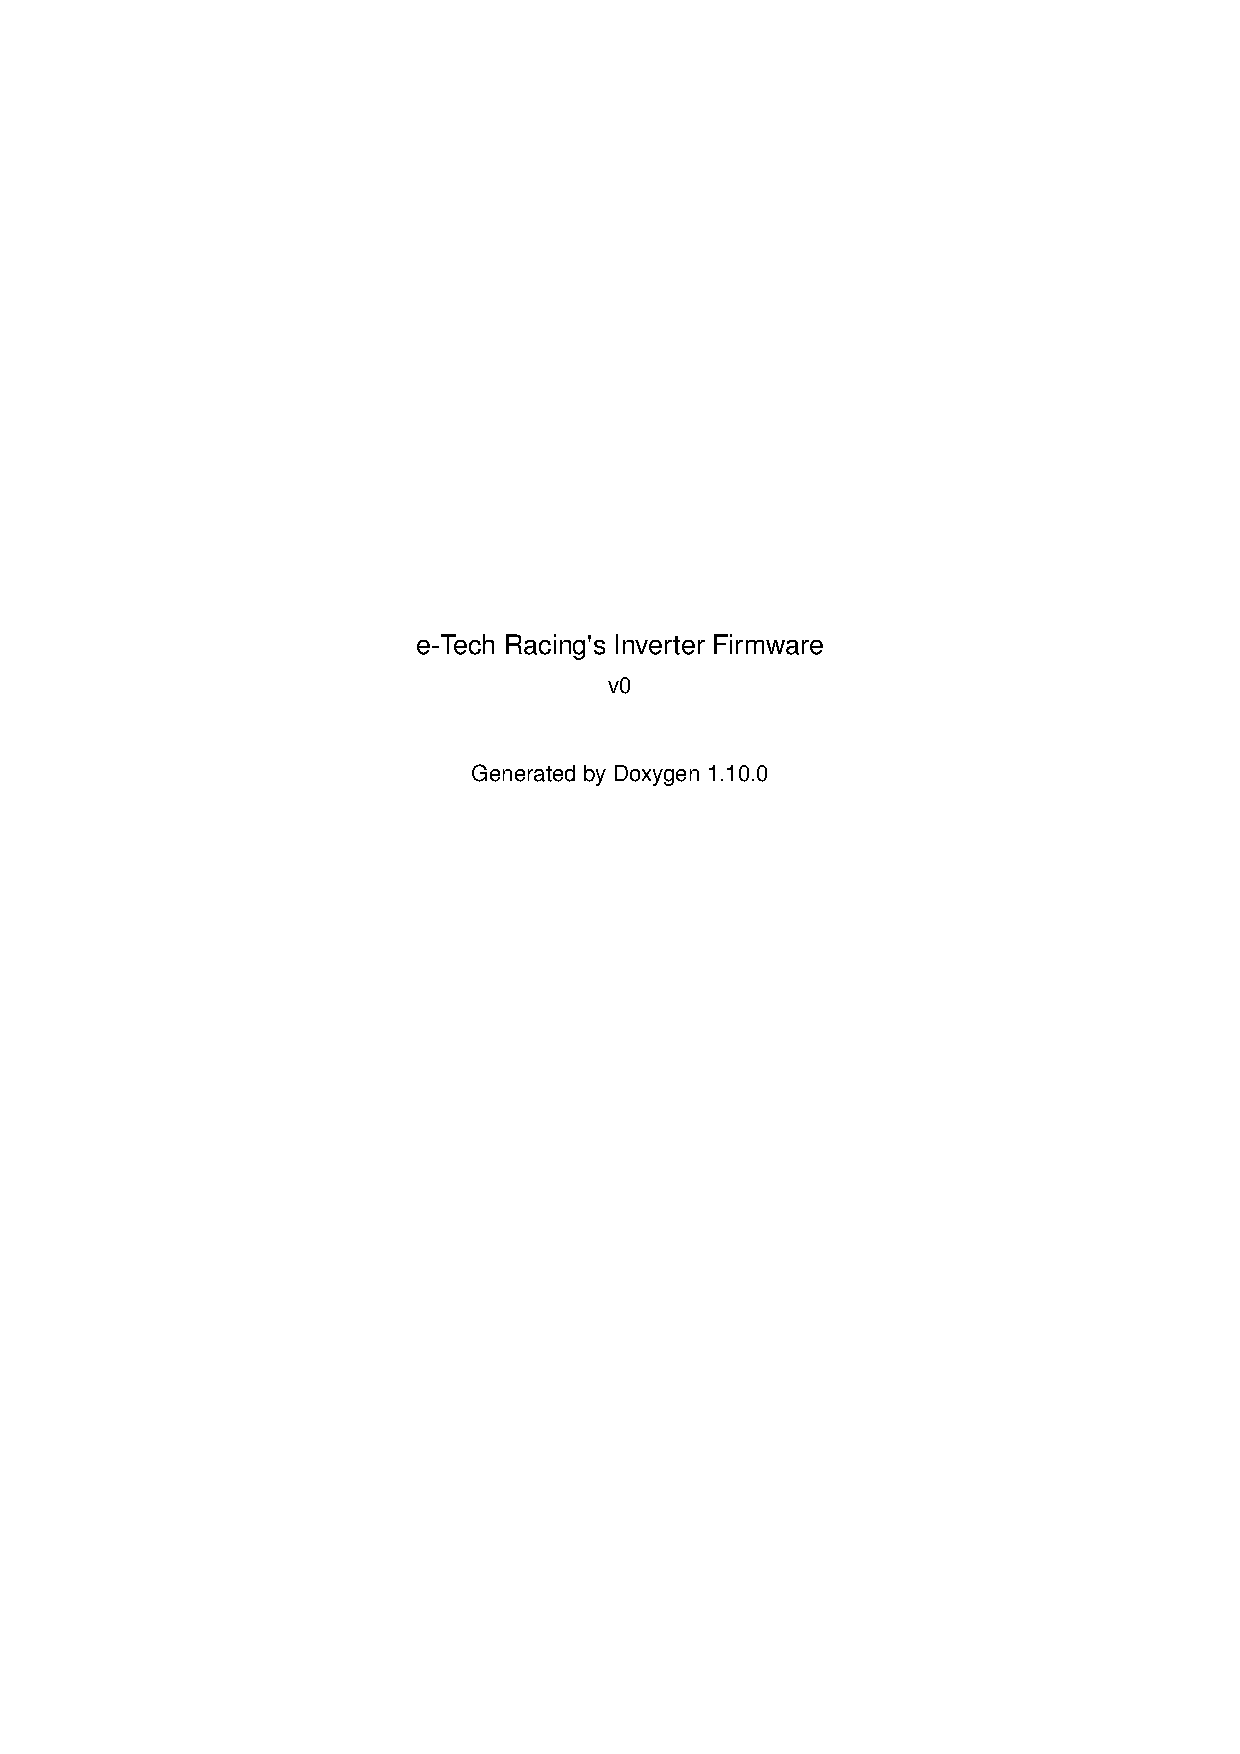
\includepdf[pages=-]{../SW/Documentation/latex/refman.pdf}
